
% This LaTeX was auto-generated from MATLAB code.
% To make changes, update the MATLAB code and republish this document.

\documentclass{article}
\usepackage{graphicx}
\usepackage{color}

\sloppy
\definecolor{lightgray}{gray}{0.5}
\setlength{\parindent}{0pt}

\begin{document}

    
    \begin{verbatim}
%set up memory
links = zeros(6,4);
A = ones(4,4,length(links(:,1)));
T = ones(4,4,length(links(:,1)));

%go to home
theta = [0 0 0 0 0 0];
links(1,:) = [ 75 90 330 theta(1)];
links(2,:) = [ 300 0 0 theta(2)];
links(3,:) = [ 75 90 0 theta(3)];
links(4,:) = [ 0 -90 320 theta(4)];
links(5,:) = [ 0 90 0 theta(5)];
links(6,:) = [ 0 0 80 theta(6)];

%get the A and T matrix
A = getA(links)
T = getT(A)

%plot
figure(1);
title('home position')
plotArm(T)


%go to work position
theta = [0 75 30 135 -45 60];
links(1,:) = [ 75 90 330 theta(1)];
links(2,:) = [ .300 0 0 theta(2)];
links(3,:) = [ 75 90 0 theta(3)];
links(4,:) = [ 0 -90 320 theta(4)];
links(5,:) = [ 0 90 0 theta(5)];
links(6,:) = [ 0 0 80 theta(6)];
A = getA(links)
T = getT(A)

%plot the work position
figure(2)
plotArm(T)
title('work position')
\end{verbatim}

        \color{lightgray} \begin{verbatim}
A(:,:,1) =

    1.0000         0         0   75.0000
         0    0.0000   -1.0000         0
         0    1.0000    0.0000  330.0000
         0         0         0    1.0000


A(:,:,2) =

     1     0     0   300
     0     1     0     0
     0     0     1     0
     0     0     0     1


A(:,:,3) =

    1.0000         0         0   75.0000
         0    0.0000   -1.0000         0
         0    1.0000    0.0000         0
         0         0         0    1.0000


A(:,:,4) =

    1.0000         0         0         0
         0    0.0000    1.0000         0
         0   -1.0000    0.0000  320.0000
         0         0         0    1.0000


A(:,:,5) =

    1.0000         0         0         0
         0    0.0000   -1.0000         0
         0    1.0000    0.0000         0
         0         0         0    1.0000


A(:,:,6) =

     1     0     0     0
     0     1     0     0
     0     0     1    80
     0     0     0     1


T(:,:,1) =

    1.0000         0         0   75.0000
         0    0.0000   -1.0000         0
         0    1.0000    0.0000  330.0000
         0         0         0    1.0000


T(:,:,2) =

    1.0000         0         0  375.0000
         0    0.0000   -1.0000         0
         0    1.0000    0.0000  330.0000
         0         0         0    1.0000


T(:,:,3) =

    1.0000         0         0  450.0000
         0   -1.0000   -0.0000         0
         0    0.0000   -1.0000  330.0000
         0         0         0    1.0000


T(:,:,4) =

    1.0000         0         0  450.0000
         0    0.0000   -1.0000   -0.0000
         0    1.0000    0.0000   10.0000
         0         0         0    1.0000


T(:,:,5) =

    1.0000         0         0  450.0000
         0   -1.0000   -0.0000   -0.0000
         0    0.0000   -1.0000   10.0000
         0         0         0    1.0000


T(:,:,6) =

    1.0000         0         0  450.0000
         0   -1.0000   -0.0000   -0.0000
         0    0.0000   -1.0000  -70.0000
         0         0         0    1.0000


A(:,:,1) =

    1.0000         0         0   75.0000
         0    0.0000   -1.0000         0
         0    1.0000    0.0000  330.0000
         0         0         0    1.0000


A(:,:,2) =

    0.2588   -0.9659         0    0.0776
    0.9659    0.2588         0    0.2898
         0         0    1.0000         0
         0         0         0    1.0000


A(:,:,3) =

    0.8660   -0.0000    0.5000   64.9519
    0.5000    0.0000   -0.8660   37.5000
         0    1.0000    0.0000         0
         0         0         0    1.0000


A(:,:,4) =

   -0.7071   -0.0000   -0.7071         0
    0.7071   -0.0000   -0.7071         0
         0   -1.0000    0.0000  320.0000
         0         0         0    1.0000


A(:,:,5) =

    0.7071    0.0000   -0.7071         0
   -0.7071    0.0000   -0.7071         0
         0    1.0000    0.0000         0
         0         0         0    1.0000


A(:,:,6) =

    0.5000   -0.8660         0         0
    0.8660    0.5000         0         0
         0         0    1.0000   80.0000
         0         0         0    1.0000


T(:,:,1) =

    1.0000         0         0   75.0000
         0    0.0000   -1.0000         0
         0    1.0000    0.0000  330.0000
         0         0         0    1.0000


T(:,:,2) =

    0.2588   -0.9659         0   75.0776
    0.0000    0.0000   -1.0000    0.0000
    0.9659    0.2588    0.0000  330.2898
         0         0         0    1.0000


T(:,:,3) =

   -0.2588   -0.0000    0.9659   55.6662
    0.0000   -1.0000   -0.0000    0.0000
    0.9659    0.0000    0.2588  402.7342
         0         0         0    1.0000


T(:,:,4) =

    0.1830   -0.9659    0.1830  364.7625
   -0.7071    0.0000    0.7071   -0.0000
   -0.6830   -0.2588   -0.6830  485.5563
         0         0         0    1.0000


T(:,:,5) =

    0.8124    0.1830    0.5536  364.7625
   -0.5000    0.7071    0.5000   -0.0000
   -0.3000   -0.6830    0.6660  485.5563
         0         0         0    1.0000


T(:,:,6) =

    0.5647   -0.6121    0.5536  409.0507
    0.3624    0.7866    0.5000   40.0000
   -0.7415   -0.0817    0.6660  538.8344
         0         0         0    1.0000

\end{verbatim} \color{black}
    
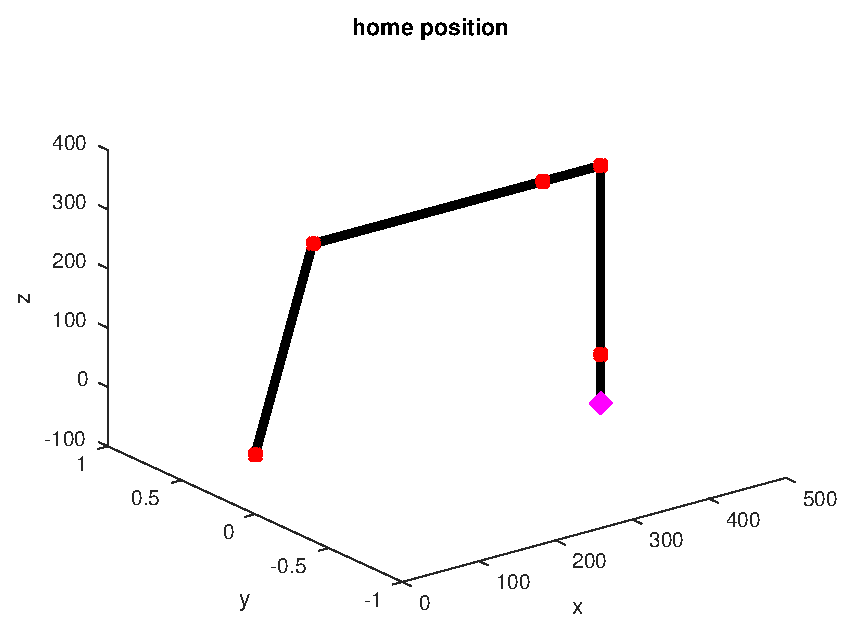
\includegraphics [width=4in]{Fanuc_01.eps}

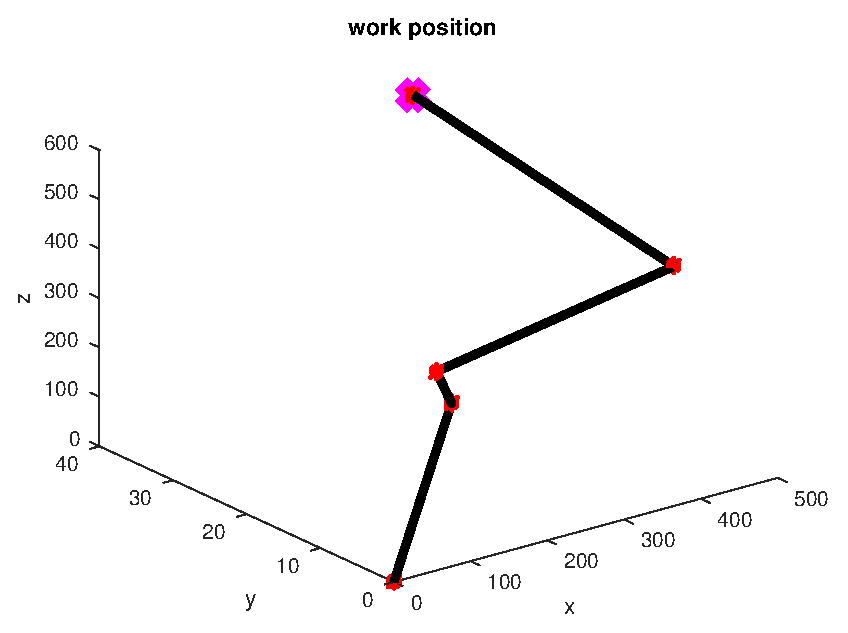
\includegraphics [width=4in]{Fanuc_02.eps}



\end{document}
    
